% !TEX output_directory=output
\documentclass{beamer}

\usepackage[beamer]{kaufman}

\bibliography{../refs.bib}
\graphicspath{{../graphics/}}

\title{Hamiltonian Engineering via Reinforcement Learning}
\author{Will Kaufman}
\institute{Ramanathan Group \\ Dartmouth College}

\titlegraphic{\includegraphics[height=.1\textheight]{LonePine.pdf}}

\begin{document}

\frame{\titlepage}

\begin{frame}
\frametitle{Table of Contents}
\tableofcontents
\end{frame}

\section{Hamiltonian engineering}

\begin{frame}
\frametitle{Hamiltonian engineering}

Hamiltonian engineering seeks to control the system's evolution so that it appears to evolve under a target ``effective'' Hamiltonian.

\begin{equation}
    H(t) = H_\text{system} + H_\text{control}(t)
\end{equation}

\begin{equation}\label{eq:strob_measure}
    \rho(Nt_c) = U_\text{target}(Nt_c) \rho(0) U_\text{target}^\dagger(Nt_c)
\end{equation}

\pause

In NMR \cite{1976ii}\dots

\begin{align}\label{eq:ham_spin}
    H_\text{system} &= \sum_i \delta_i I_z^i + \sum_{i,j} d_{ij} \left( 3I_z^iI_z^j - \mathbf{I^i} \cdot \mathbf{I^j} \right)
    = H_\text{CS} + H_\text{D} \\
    H_\text{control}(t) &= -B_1(t) \sum_i \gamma_n^i I_x^i
\end{align}

\end{frame}

\section{Previous approaches}

\begin{frame}
\frametitle{Average Hamiltonian theory}

Average Hamiltonian theory is one approach to solving the Hamiltonian engineering problem
\cite{PhysRev.175.453}.
If a pulse sequence with cycle time is both cyclic and periodic
\cite{gerstein-dybowski}
\begin{align}\label{eq:AHT_conditions}
    U_\text{rf}(t_c) &= T\exp \left(
        -i \int_0^{t_c} H_\text{rf}(t) dt \right) = \pm \identity
        & \text{(cyclic)} \\
    H_\text{rf}(t) &= H_\text{rf}(t + Nt_c) & \text{(periodic)}
\end{align}
then, using the Magnus Expansion, the propagator can be given by
\begin{align}\label{eq:AHT_average}
    U(t_c) &= \exp\left( -i t_c (\overline{H}^{(0)} +
        \overline{H}^{(1)} + \dots) \right) \\
    \overline{H}^{(0)} &= 1/t_c \int_0^{t_c}
        U_\text{rf}(t) H_\text{int} U_\text{rf}^\dagger(t) dt
\end{align}

\end{frame}

\begin{frame}
\frametitle{Average Hamiltonian theory: examples}

To engineer a target Hamiltonian $H_t$, the pulse sequence is chosen so that $\overline{H}^{(0)} = H_t$. Higher-order terms $\overline{H}^{(1)}, \overline{H}^{(2)}, \dots$ can also be considered (e.g. symmetrization).

\begin{table}
\centering
\scalebox{.8}{
\begin{tabular}{c c c}
    Name & Pulse sequence (left to right) & $\overline{H}^{(0)}$ \\
    \hline
    WHH-4 \cite{PhysRevLett.20.180} &
        $\tau, \overline{X}, \tau, Y, 2\tau, \overline{Y}, \tau, X, \tau$ &
        $\frac{1}{3} \sum_i \delta_i \left( I_x^i + I_y^i + I_z^i \right)$ \\
    MREV-8 \cite{mansfield1971symmetrized} & \vtop{\hbox{\strut
        $\tau, \overline{X}, \tau, Y, 2\tau, \overline{Y}, \tau, X, 2\tau,$
        }\hbox{\strut
        $X, \tau, Y, 2\tau, \overline{Y}, \tau, \overline{X}, \tau$
        }} &
        $\frac{1}{3} \sum_i \delta_i \left( I_x^i + I_z^i \right)$ \\
    HoRD-qubit-5 \cite{O_Keeffe_2019} & \vtop{\hbox{\strut
        $\tau, Y, \tau, X^2, \tau, X Y \overline{X}^2,$
        }\hbox{\strut
        $\tau, \overline{X} Y \overline{X}, \tau, Y X, \tau$
        }} &
        $1/3 \sum_i I_z^i$ \\
    \hline
\end{tabular}
}
\end{table}


Pulse sequences for dipolar decoupling of spin-1 systems exist \cite{PhysRevLett.119.183603, O_Keeffe_2019}.

\end{frame}

\begin{frame}
\frametitle{Average Hamiltonian theory: benefits and limitations}

\begin{itemize}
    \item Analytically tractable
    \item Account for finite-width pulses
    \item Can characterize terms in average Hamiltonian
    \pause
    \item Only tractable for lowest-order terms
    \item Enforced structure on pulse sequences
\end{itemize}

\end{frame}

\begin{frame}[allowframebreaks]
\frametitle{Gradient ascent pulse engineering (GRAPE)}

The control Hamiltonian is parametrized by amplitudes $u_k(t)$ so that
\begin{equation}
    H_\text{control}(t) = \sum_k u_k(t) H_k
\end{equation}

And a performance function $\Phi$ measures the overlap with a target operator
\begin{align*}
    \Phi_0 &= \Tr{C^\dagger \rho(t_\text{cyc})} &
        \text{ (Hermitian operator transfer)} \\
    \Phi_3 &= \Re \Tr{U_\text{target}^\dagger U(t_\text{cyc})} &
        \text{ (unitary synthesis)}
\end{align*}
$\Phi$ is maximized by the following amplitude update rule
\begin{equation}
    u_k(j) \to u_k(j) + \epsilon \frac{\delta \Phi}{\delta u_k(j)}
\end{equation}

\begin{itemize}
    \item Easily extended to range of parameters for robustness
    \item Algorithm depends on initial random amplitudes, duration $t_\text{cyc}$, and discretization $N = \Delta t/t_\text{cyc}$
    % \item Not well-suited for continuous-time problems
    % TODO include above?
\end{itemize}

\end{frame}

\section{Reinforcement learning as alternative approach}

\begin{frame}
\frametitle{Reinforcement learning paradigm}

\begin{quote}
    Reinforcement learning is learning what to do--how to map situations to actions--so as to maximize a numerical reward signal. \cite{sutton2018reinforcement}
\end{quote}

\begin{figure}
    \centering
    \scalebox{.5}{
    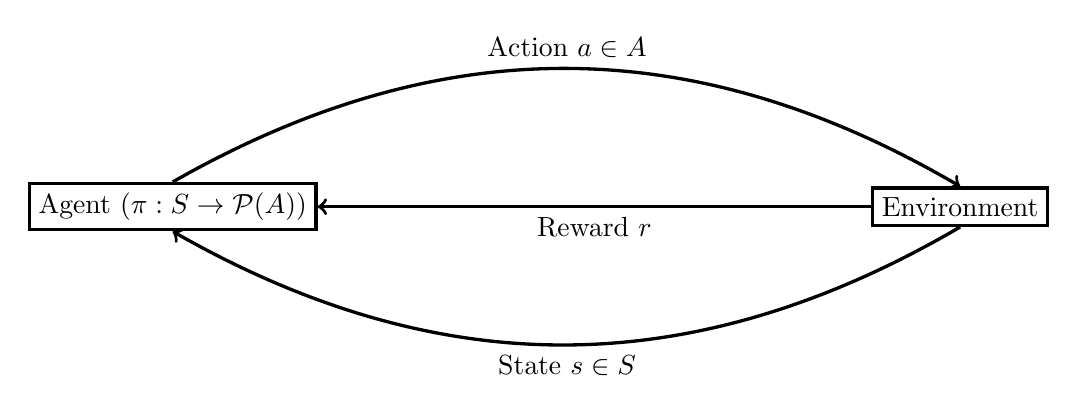
\begin{tikzpicture}[->, very thick]
         %nodes
         \node[draw] at (-5,0) (agent) {Agent ($\pi: S \to \mathcal{P}(A)$)};
         \node[draw] at (5,0) (env) {Environment};
         \path
             (agent.north) edge[bend left=30] node[above] {Action $a \in A$} (env.north)
             (env.south) edge[bend left=30] node[below] {State $s \in S$} (agent.south)
             (env.west) edge node[below] {Reward $r$} (agent.east);
    \end{tikzpicture}
    }
    %\caption{The general reinforcement learning paradigm.}
    \label{fig:RL}
\end{figure}

Different from supervised learning, where labeled data trains a model.

% \emph{Many} variations of reinforcement learning algorithms.

\end{frame}

\begin{frame}
\frametitle{RL Definitions}

\begin{itemize}
    \item State space $S$; all possible states of the environment
    \item Action space $A$: all possible actions that can be performed
    \item Total return $R_t$: sum of all rewards from time $t$ to end of episode (length $T$)
    \begin{equation}\label{eq:return}
        R_t = \sum_{k=t}^T r_k
    \end{equation}
    \pause
    \item Stochastic policy $\pi: S \to \mathcal{P}(A)$:
        maps from states to probability distributions over actions (also written $\pi(a|s)$)
    \item State value $V^\pi:S \to \R$: expected return from state following policy $\pi$
    % \item State-action value $Q^\pi: S \times A \to \R$: expected return from state and performing action, then following policy $\pi$
\end{itemize}

\end{frame}

\begin{frame}
\frametitle{Actor-critic methods}

A ``critic'' learns the value function $V^\pi_\phi$, and an ``actor'' learns the policy function $\pi_\theta$ \cite{sutton2018reinforcement}.

\begin{align}\label{eq:loss_fns}
    L(\phi) &= \sum_i (\hat{R}_i - V^\pi_\phi(s_i))^2 \\
    L(\theta) &= -\sum_i (\hat{R}_i - V^\pi_\phi(s_i))
        \ln \pi_\theta(a_i|s_i)
\end{align}

$\hat{R}_i - V^\pi_\phi(s_i)$ is called the \emph{advantage} $A_i$.

\pause

\begin{itemize}
    \item Can be trained ``online'' (one experience at a time) or ``offline'' using replay buffer
    \item Susceptible to local minima
\end{itemize}

\end{frame}

\begin{frame}
\frametitle{Evolutionary reinforcement learning}

Hybrid algorithm that uses both policy gradient (PG) and evolutionary algorithms (EA).

\begin{figure}
    \centering
    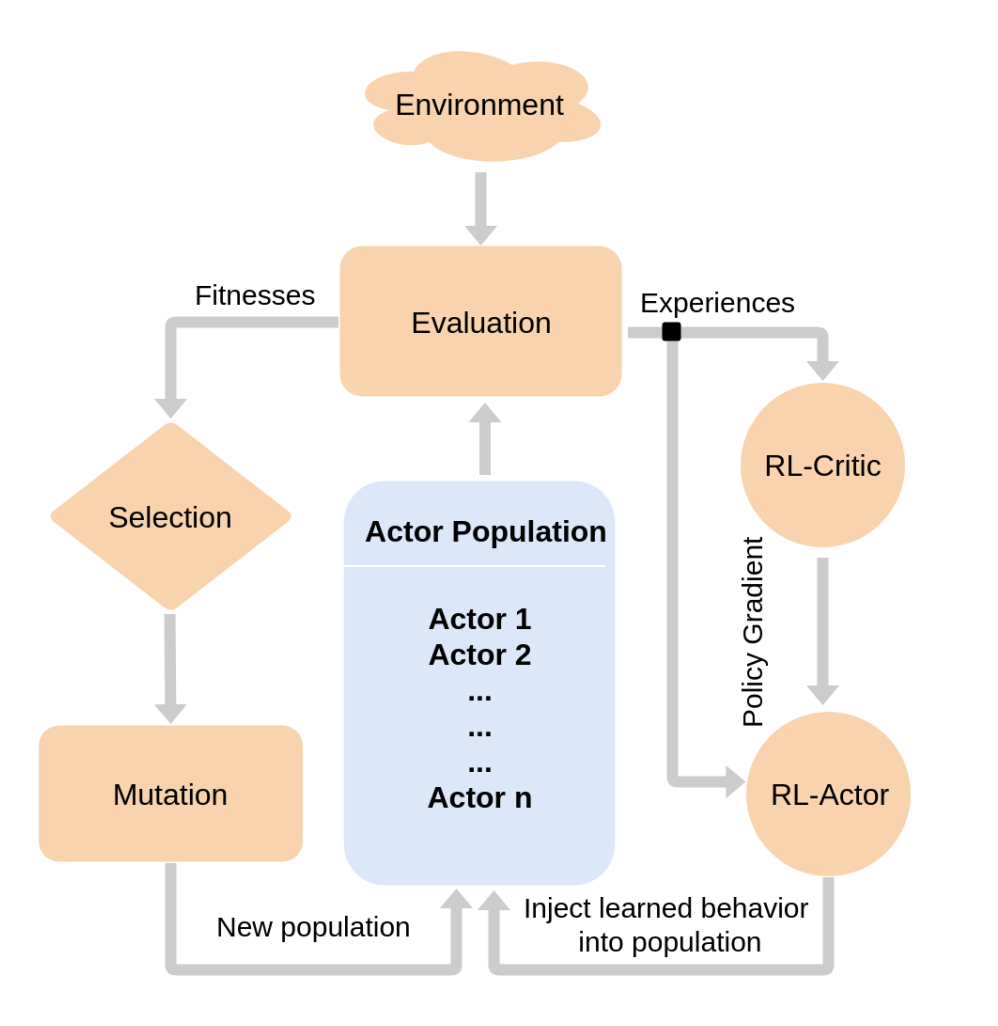
\includegraphics[height=0.6\textheight]{ERL.png}
    \caption{Reproduced from \cite{khadka2018evolutionguided}.}
    \label{fig:ERL}
\end{figure}
\cite{khadka2018evolutionguided}

\begin{itemize}
    \item Information flows between EA and PG components
    \item Diverse exploration of action space
\end{itemize}

\end{frame}

\begin{frame}
\frametitle{Applying RL to Hamiltonian engineering}

\begin{table}
\label{tab:rl_ham}
\scalebox{.9}{
\begin{tabular}{c c c}
    RL concept & Hamiltonian engineering & Code representation \\
    \hline
    Action & Unitary operator & Indicator vector \\
    State & Propagator $U(t)$ & Sequence of action vector \\
    Reward & Unitary operator fidelity &
        $r = -\log \left( 1 - \Re{
            \frac{\Tr{U_\text{target}^\dagger U(t)}}{\Tr{\identity}}
        } \right)$ \\
\end{tabular}
}
\end{table}

% TODO include example of what it looks like...

\end{frame}

\section{Results}

\begin{frame}[allowframebreaks]
\frametitle{Hyperparameter search and algorithm performance}

Many hyperparameters to tune for ERL model
\begin{itemize}
    \item Learning rates (actor and critic)
    \item Neural network architecture (RNN layer type, depth, width, activation functions)
    \item Gradient update frequency (online learning or experience replay)
    \item \dots
\end{itemize}

Hyperparameter combinations so far haven't led to consistent policy convergence.
\begin{figure}
    \centering
    \includegraphics[width=.9\textwidth]{2020-06-23/popFitnesses-002.png}
    \label{fig:popFitnesses}
\end{figure}

% TODO continue here...

\end{frame}

\begin{frame}
\frametitle{Candidate pulse sequences}

Although ERL algorithm hasn't consistently converged to good policies, several candidate pulse sequences have been identified.

\begin{table}
    \label{tab:candidates}
    \begin{tabular}{c c}
        Number & Pulse sequence (left to right) \\
        \hline
        % note that there was another pulse sequence that
        % turned out to be bad, so 2,3,4 were renumbered as 1,2,3
        1 & $\tau, \overline{X}, Y, \tau, \overline{X}, \tau, \overline{Y}, \overline{X}^2$ \\
        2 & $\overline{X}, \tau, \overline{X}, \tau, \overline{Y}, X$ \\
        3 & $X, \overline{Y}, \overline{X}, \tau, X, \overline{Y}^2, \tau, $
            $Y, \tau, \overline{X}, Y^2, X^2$ \\
    \end{tabular}
\end{table}

% TODO
% general evaluation strategy (compare to WHH-4, MREV-8)
% compare on similar timeframe
% robustness?
% simulation parameters

\end{frame}

\begin{frame}
\frametitle{Candidate 1 pulse sequence performance}

\begin{figure}
    \centering
    \includegraphics[height=.8\textheight]{2020-06-23/reward_hist-2.pdf}
    \label{fig:candidate_1}
\end{figure}

\end{frame}

\begin{frame}
\frametitle{Candidate 2 pulse sequence performance}

\begin{figure}
    \centering
    \includegraphics[height=.8\textheight]{2020-06-23/reward_hist-3.pdf}
    \label{fig:candidate_2}
\end{figure}


\end{frame}

\begin{frame}
\frametitle{Candidate 3 pulse sequence performance}

\begin{figure}
    \centering
    \includegraphics[height=.8\textheight]{2020-06-23/reward_hist_N4_coupling1e4.pdf}
    \label{fig:candidate_3}
\end{figure}

\end{frame}

\section{Next steps}

\begin{frame}
\frametitle{Improvements to RL algorithm}

\begin{itemize}
    \item Convergence to optimal policy
    \item Robustness against errors
    \item Algorithm efficiency
    \item Variety of target Hamiltonians
    \item Explore GRAPE-like implementation
    \pause
    \item Change algorithm to include MCTS (similar to AlphaZero)
\end{itemize}

\end{frame}

\begin{frame}
\frametitle{Experimental verification of candidate pulse sequences}

\begin{itemize}
    \item Measures of performance in experiments
    \item % TODO more here???
\end{itemize}

\end{frame}

\begin{frame}[allowframebreaks]
\frametitle{Bibliography}

\printbibliography

\end{frame}






\end{document}
